\documentclass[%
	fontsize=11pt,% bigger font
	paper=a4,% paper size
	pagesize,% set pagesize in PDF
	twoside=false,% =oneside
	listof=totoc,%add list of figures to toc
	draft% TODO remove this!
]{scrbook}

%---------------------------------------
%---------PACKAGES----------------------
%---------------------------------------

% language
\usepackage[english]{babel}

% font config
\usepackage{libertine}
\usepackage[T1]{fontenc}

% microtype
\usepackage[
	activate={true,nocompatibility},% activate protrusion and expansion
	final,% enable microtype; use "draft" to disable
	tracking=true,% activate these techniques
	kerning=true,% -''-
	spacing=nonfrench,% activate and supress warning
	factor=1100,% add 10% to the protrusion amount (default is 1000)
	stretch=10,% reduce stretchability/shrinkability (default is 20/20)
	shrink=10% -''-
]{microtype}

% links
\usepackage{hyperref}

% math
\usepackage{amsmath}
\usepackage{amssymb}

% graphics
\usepackage{tikz}
\usepackage{tikz-3dplot}
\usepackage{pgfplots}

% glossar
% dep: hyperref
\usepackage[
	toc% add to toc
]{glossaries}

% bibtex
% dep: hyperref
\usepackage[
	backend=biber,% nice fast backend
	style=alphabetic% how the shortcuts should look like
]{biblatex}

% units
% dep: amssymb
\usepackage{siunitx}

% subfigures
\usepackage{subfig}

% list of symbols
\usepackage[intoc]{nomencl}

% TODO remove this!
% debug packages
\usepackage{blindtext}


%---------------------------------------
%---------SETTINGS----------------------
%---------------------------------------

% general informaion
\title{Some funny words}
\author{Marco Neumann}

% color
\definecolor{colcontrast}{RGB}{40,100,40}
\definecolor{colcontrast2}{RGB}{40,40,100}
\definecolor{colcontrast3}{RGB}{80,20,80}
\definecolor{colcontrast4}{RGB}{80,80,20}

% links
\hypersetup{
	colorlinks,% colored text instead of borders
	linkcolor=black,% black inter document links
	urlcolor=black,% black urls
	citecolor=black,% black cite
	final% also work in draft mode, TODO remove this!
}

% tikz
\usetikzlibrary{
	arrows,
	positioning
}
\tikzset{
	>=stealth',
	axis/.style={->, very thick, >=stealth'},
	graphedge/.style={ultra thick},
	graphnode/.style={circle, draw}
}
\newcommand*\circled[1]{\tikz[baseline={($(char.south) + (0,0.5pt)$)}]{
	\node[shape=circle,draw,inner sep=0.5pt,font=\tiny,thick] (char) {\textsf{#1}};}}

% bibtex
\addbibresource{citiation.bib}

% list of figures
\captionsetup{lofdepth=2}

% list of symbols
\makenomenclature
\renewcommand{\nomname}{List of Symbols}

% math macros
\newcommand{\set}[1]{\mathbb{#1}}
\newcommand{\card}[1]{\left|#1\right|}

% calculation helper
\newcommand{\mycalc}[2]{
	\pgfkeys{/pgf/fpu, /pgf/fpu/output format=fixed}
	\pgfmathparse{#2}
	\edef#1{\pgfmathresult}
	\pgfkeys{/pgf/fpu=false}
}

%---------------------------------------
%---------LIST OF SYMBOLS---------------
%---------------------------------------
\nomenclature{$D$}{Set of all dimenions}
\nomenclature{$\card{D}$}{Total number of dimenions}
\nomenclature{$N$}{Set of all objects}
\nomenclature{$\card{N}$}{Total number of objects}


%---------------------------------------
%---------GLOSSARY----------------------
%---------------------------------------

\newglossaryentry{random number generator}
{
	name={Random Number Generator},
	description={Generates random numbers}
}

\newacronym{rng}{RNG}{\glslink{random number generator}{Random Number Generator}}

\makeglossaries% build glossary
\glsunsetall% fix acronyms


\begin{document}

\frontmatter
\maketitle
\tableofcontents

\mainmatter
\chapter{Designing a high perfomance algorithm}
To handle current and future big datasets a special approach is required. In this chapter, I will design a high perfomance algorithm that is able to handle this task. The main goal is a method that does not beat the comlexity of $\mathcal{O} ( \card{D} \cdot \card{N} \cdot \log{\card{N}} + \card{D}^2 \cdot \card{N} )$. This complexity is a good upper bound. It combines the bounds of two different task. The first one is the preprocessing and structure detection of all objects in all dimensions. $O\left( D \cdot N \right)$ would be enough to normalize the data, but $O\left( D \cdot N \cdot \log{N} \right)$ allowes some better methods like sorting. The second part is the detection of relations between all dimensions, which could be done in $O\left( D^2 \right)$. Because reducing the dimenions to a fixed set of features does honor a non fixed number of elements, a good method needs $O\left( D^2 \cdot N \right)$.

\section{Optimize graph structure}
\begin{figure}
	\caption{Different subspaces from different graph preprocessing}
	\label{fig:opt_graph}
	\centering
	\subfloat[\label{subfig:opt_graph1}Too many subspaces]{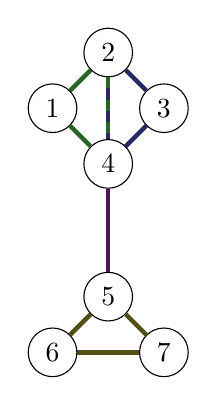
\begin{tikzpicture}
	\node[graphnode] (1) {1};
	\node[graphnode] (2) [above right of=1] {2};
	\node[graphnode] (3) [below right of=2] {3};
	\node[graphnode] (4) [below right of=1] {4};
	\node[graphnode] (5) [below=30pt of 4] {5};
	\node[graphnode] (6) [below left of=5] {6};
	\node[graphnode] (7) [below right of=5] {7};

	\path[graphedge, color=colcontrast]
		(1) edge (2)
			edge (4)
	;

	\path[graphedge, color=colcontrast2]
		(3) edge (2)
			edge (4)
	;

	\path[graphedge, color=colcontrast, dash pattern=on 4pt off 4pt]
		(2) edge (4)
	;

	\path[graphedge, color=colcontrast2, dash pattern=on 4pt off 4pt, dash phase=4pt]
		(2) edge (4)
	;

	\path[graphedge, color=colcontrast3]
		(4) edge (5)
	;

	\path[graphedge, color=colcontrast4]
		(5) edge (6)
			edge (7)
		(6) edge (7)
	;
\end{tikzpicture}

}
	\hfill
	\subfloat[\label{subfig:opt_graph2}Simple graph distance]{\input{figures/graph2.tex}}
	\hfill
	\subfloat[\label{subfig:opt_graph3}Filtered distance with $\alpha=\frac23$]{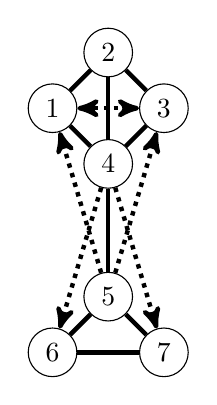
\begin{tikzpicture}
	\node[graphnode] (1) {1};
	\node[graphnode] (2) [above right of=1] {2};
	\node[graphnode] (3) [below right of=2] {3};
	\node[graphnode] (4) [below right of=1] {4};
	\node[graphnode] (5) [below=30pt of 4] {5};
	\node[graphnode] (6) [below left of=5] {6};
	\node[graphnode] (7) [below right of=5] {7};

	\path[graphedge]
		(2) edge (1)
			edge (3)
		(4) edge (1)
			edge (2)
			edge (3)
			edge (5)
		(5) edge (6)
			edge (7)
		(6) edge (7)
	;

	\path[graphedge, dotted]
		(1) edge[<->] (3)
		(5) edge[->] (1)
			edge[->] (3)
		(4) edge[->] (6)
			edge[->] (7)
	;
\end{tikzpicture}

}
	\hfill
	\subfloat[\label{subfig:opt_graph4}Bidirectional filtered distance with $\alpha=\frac23$]{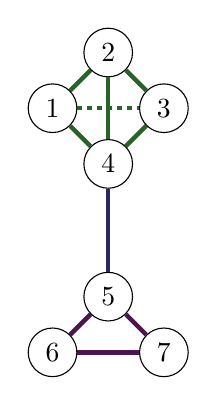
\begin{tikzpicture}
	\node[graphnode] (1) {1};
	\node[graphnode] (2) [above right of=1] {2};
	\node[graphnode] (3) [below right of=2] {3};
	\node[graphnode] (4) [below right of=1] {4};
	\node[graphnode] (5) [below=30pt of 4] {5};
	\node[graphnode] (6) [below left of=5] {6};
	\node[graphnode] (7) [below right of=5] {7};

	\path[graphedge, color=colcontrast]
		(2) edge (1)
			edge (3)
			edge (4)
		(4) edge (1)
			edge (3)
	;

	\path[graphedge, color=colcontrast, dotted]
		(1) edge (3)
	;

	\path[graphedge, color=colcontrast2]
		(4) edge (5)
	;

	\path[graphedge, color=colcontrast3]
		(5) edge (6)
			edge (7)
		(6) edge (7)
	;
\end{tikzpicture}

}
\end{figure}


\chapter{Implementation}
For the researcher who want only get a described complexity it is sufficient to use a favorite programming languge or DBMS. But if you want to handle big data before getting to old, it is important to choose the right tools and think about some implementation details. In this chapter I want to descibe and explain my choices and would like to give you some impressions about the implementation process. Some but not all strategies can also be used for other algorithms and may be used for some other work too. I will finish the chapter with some ideas about future improvements.

\section{Choosing a programming language}
To express the designed algorithm and let the computer do the job it is necessary to write some source code. There are dozend different programming languages out there and every language has its own pros and cons.

A simple and very comfortable choice is a language with a good buildin runtime library.\footnote{What ``good'' means in this context depends on the algorithm that you want to implement and the operations you need.} Python or Matlab is a good choice. Please notice that SQL or other database bound languages are not very portable and suffer when it comes to debugging and flexibility. If the language provided a embedded mathematic system like Matlab, it is easy to map the theoretical terms to the language. Matrix support makes it easy to handle big amounts of data. The key feature of the language should be syntax that does not produce much boiler plate. This is one point where script languages are very good, but lanuages like Java are not. C++ provides a short syntax for many things, but suffers like many other compiled langues when you want a comfortable environment. Typesafety is another point that can be useful because it allowes you to tackle many bugs before you waste your time for runtime tests.

The next point is a good library support for things that the choosen language does not provide. Matrix operations require a special library, escecially if you want to invert or decomposit them. High precision floating point operations and big integer calculation needs a different library. Parsing, code managment or special IO operations is another topic. Also notice that I don't mean the standard library. A well tested and documented library is required. For example NumPy if you use Python.

In addition to the things you as the author and primary user of the implementation finds useful are the problems your team or the consumers need. An exotic language\footnote{Don't know what I mean? Go and find something about APL} may be very cool but if nobody can read your code, your research result doesn't help someone. This does not mean that you have to stuck in old good Java or COBOL, but it means that you have to think about the innovation you want to use. Also think about portability, future development and safety of the language. Safety is important if you don't want to risk the data of your institution or the consumers. You may think that the implementation is only for internal tests but if your results are good it can be the case that your code will be published or used by other persons. Even if low level languages can be insecure when doing unchecked memory operations, also interpreted languages have many weaknesses.

You may ask where this all have to do with high perfomance. The simple answer is: nothing. They make your life easier, but do not provide a fast implementation. So the most important point for my work is performance. And this kills the most high level languages, because they do not provide a fine grained control about data allocation, movement and copying. Even the object overhead of languages like Java and naiv C++ is too big. I had to strip down the calculation core to a simple low level core. But I do not want to loose all high level features. In my eyes, there is currently only one languages that provides this schizophrenia: handcrafted and well written C++. I will give you some rules about hints about the language specific methods in the next section.

\section{Special C++ tips}
C++ can be used in many different ways, depending on your background, the interfaces you want to use or have to provide and the attributes your program should have. As most other programming languages out there, C++ is avaiable in different standarts and the compiler and STL support differs. One of the best collections of tips for good programming style is \cite{effectiveCpp}. Furthermore I used the new C++11 standard which brings makes many code sections easier to read and more C++ stylish rather than C based. It also avoids many boiler blade an manual memory management. Templates may be the most hated but most also most loved and most essential features of C++. I used them when I find it useful. Some calculations are written in C style because in some cases, the object overhead was to high. Because of the usage of new C++11 featues, the resulting code only compiles with newer versions of GCC and Clang. Microsoft and Intel compilers are not suppported at the time of the writing.

\section{Avoiding reinventing the wheel}
The STL already provides useful tools that makes programmers life much easier. But it does not provide high level thread operations like fork and join, system operations like memory mapped IO and fast a fast parser library. C++ has a special collection of well designed and reviewed libraries that are note yet a part of the STL: The Boost C++ Libraries. They provide two of the three libraries I was looking for -- the Boost Interprocess library, which implements memory mapped IO and the Spirit V2 library which is a special set of function and templates for parser writing. For high level multi core operations I use another well known library: the TBB, which is designed and published by Intel. All libraries are open source and free which enables researcher to use them for their work.

\chapter{How to beat the system}
The method described in this thesis has some weaknesses. I will construct a dateset, which is not processed very well and I will discuss, why this type of data is not very common.

\section{Constructing a special dataset}\label{sec:constr}
Consider the following a dataset, that is made of many random points $(x, y, z) \in \left[0, 1\right)^3$, that satisfy the following constraint:
\begin{equation}\label{eq:beat}
	(x + y + z) \bmod 1 = 0
\end{equation}
The points are uniform distributed if you project them on one or two dimensions. But if you calculate the three dimensional distribution, the points do not show a uniform distribution. (see Figure~\ref{fig:beat}). Because the generated points have two degrees of freedom, the two dimensional distribution test will fail. It is also possible to generate datasets with even more degrees of freedom using the same technique.\footnote{You may not be able to imagine datasets with more than three dimensions. For 4 dimensions, you find some help: \url{http://crepererum.github.io/brain4D/\#constructed}}
\begin{figure}
	\caption{Situation described in Equation~\ref{eq:beat}}
	\label{fig:beat}
	\subfloat[\label{subfig:beat1}1D views]{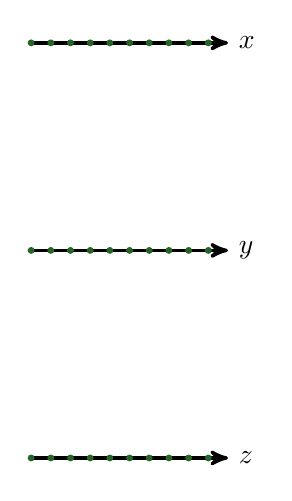
\begin{tikzpicture}[scale = 5.0]
	\foreach \name [count=\d from 0] in {x,y,z} {
		\begin{scope}[yshift=-\d*15]
			\begin{scope}[scale=0.5]
				\draw[axis] (0,0) -- (1,0) node[right]{$\name$};
				\foreach \x in {0,...,9} {
					\fill[colcontrast] (\x/10,0) circle(0.5pt);
				}
			\end{scope}
		\end{scope}
	}
\end{tikzpicture}

}
	\hfill
	\subfloat[\label{subfig:beat2}2D views]{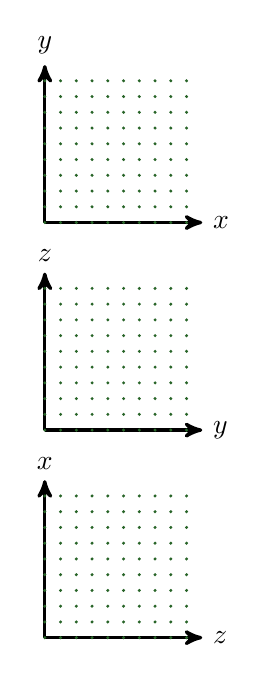
\begin{tikzpicture}[scale = 5.0]
	\foreach \namefirst/\namesecond [count=\d from 0] in {x/y,y/z,z/x} {
		\begin{scope}[yshift=-\d*15]
			\begin{scope}[scale=0.4]
				\draw[axis] (0,0) -- (1,0) node[right]{$\namefirst$};
				\draw[axis] (0,0) -- (0,1) node[above]{$\namesecond$};
				\foreach \x in {0,...,9} {
					\foreach \y in {0,...,9} {
						\fill[colcontrast] (\x/10,\y/10) circle(0.3pt);
					}
				}
			\end{scope}
		\end{scope}
	}
\end{tikzpicture}

}
	\hfill
	\subfloat[\label{subfig:beat3}3D view]{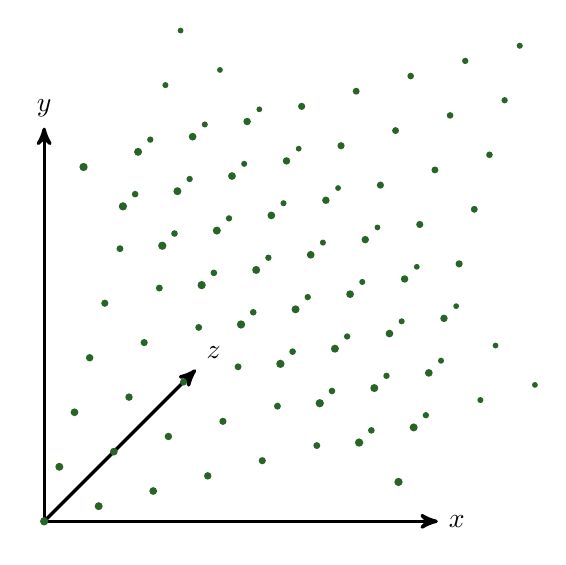
\begin{tikzpicture}[scale = 5.0]
	\begin{scope}[scale=1.0]
		\draw[axis] (0,0,0) -- (1,0,0) node[right]{$x$};
		\draw[axis] (0,0,0) -- (0,1,0) node[above]{$y$};
		\draw[axis] (0,0,0) -- (0,0,-1) node[above right]{$z$};
		\foreach \x in {0,...,9} {
			\foreach \y in {0,...,9} {
				\pgfmathsetmacro{\z}{mod(\x+\y,10)}
				\fill[colcontrast] (\x/10,\y/10,-\z/10) circle(0.3pt-0.1pt*\z/10);
			}
		}
	\end{scope}
\end{tikzpicture}

}
	\hfill
\end{figure}

The problem occures every time, when the dataset contains a subspace with $n \in \set{N}_+$ Dimensions but $m \in \left\{1,\dots,n-1\right\}$ degrees of freedom. Furthermore the dependency of each dimension on the degrees of freedom has to be equal.

\section{Handling this issue}
Because it datasets with generated dimensions are not very uncommon, I will propose a simple method to handle them. To get a good perfomance on high dimensional datasets, it is not possible to check distributions in subspaces where the size depends on the number of all dimensions. But as shown in \cite{journals/prl/SharmaP07}, a PCA can be computed in $O\left( d^2h + d^2n \right)$ where $h$ is the number of degrees of freedom. After this step, the algorithm will find the most common subspaces.


\chapter{Datasets}
High dimensional datasets are not a very common research topics. In this chapter I will describe some data sources and possible applications of the described algorithm. I also show some interpretations of subspaces in different datasets and some failed approaches of finding them. To get, isolate and preprocess the data I've used some scripts. Because I think open research should not only contain open publications but also open data sources, you can find the scripts and some notes about them online.\footnote{\url{https://github.com/crepererum/GSD}} Should you have some questions, find a bug or want to contribute, feel free to use the issue tracker or file a pull request.

\section{Audio Spectrum}
An audio spectrum can characterize the underlying material. I analyzed the songs from the following collections:
\begin{itemize}
	\item Daft Punk -- Random Access Memories (\circled{P}2013 by Daft Life, Columbia), \num{13} songs
	\item Mayday 2013 -- Never Stop Raving (\circled{C}2013 by Contor Records GmbH), \num{60} songs
\end{itemize}
I converted the audio to a sample rate of \SI{44100}{\hertz}. After it, I splitted the audio files into parts containing \num{4096} parts, applied the Hamming window and passed it to a FFT. The FFT produces a output vector with \num{4096} values, but only \num{2048} values are usable, because the spectrum should be mirrored. The values are normalized and converted to \si{\decibel}. Then I calculated the mean of \num{32} parts to supress noise, which is a common audio effect in modern music, but may also effect classical records. This mean vector has a length of \num{2048} and is written to a file. So, the mean of \num{32} parts is one data element. Figure~\ref{fig:audio} shows some of the results.
\begin{figure}
	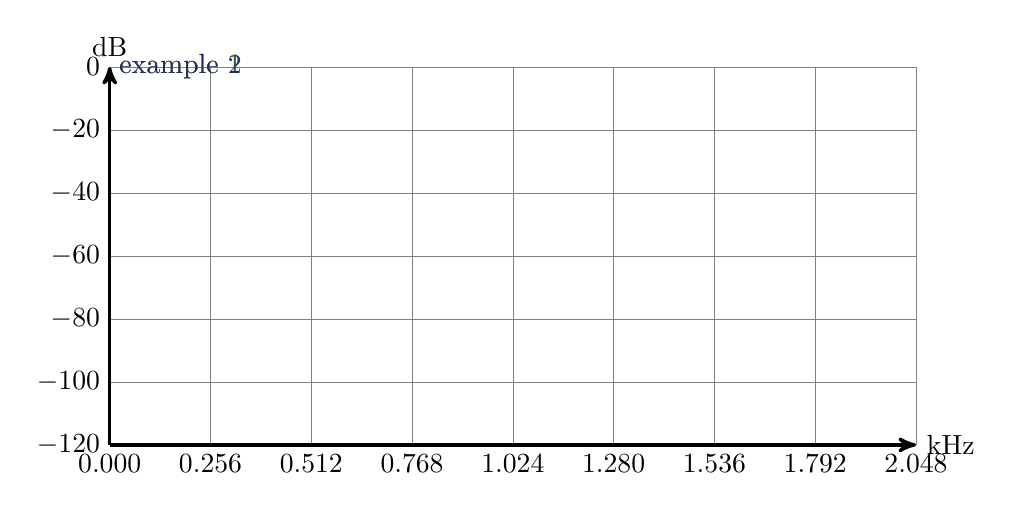
\begin{tikzpicture}
	\def\xmin{0}
	\def\xmax{2.048}
	\def\xstep{0.2}
	\def\ymin{-120}
	\def\ymax{0}
	\def\ystep{5}

	\begin{scope}[xscale=5,yscale=0.04]
		\draw[style=help lines, ystep=20, xstep=0.256] (\xmin,\ymin) grid(\xmax,\ymax);

		\foreach \x in {\xmin,0.256,...,\xmax} {
			\node at (\x,\ymin) [below]{\num[round-precision=3,round-mode=places]{\x}};
		}
		\foreach \y in {\ymin,-100,...,\ymax} {
			\node at (\xmin,\y) [left]{\num{\y}};
		}

		\draw[colcontrast] plot[smooth] file{data/audio1.dat} node[right]{example 1};
		\draw[colcontrast2] plot[smooth] file{data/audio2.dat} node[right]{example 2};

		\draw[axis] (\xmin,\ymin) -- (\xmax,\ymin) node[right]{\si{\kilo\hertz}};
		\draw[axis] (\xmin,\ymin) -- (\xmin,\ymax) node[above]{\si{\decibel}};
	\end{scope}
\end{tikzpicture}


	\caption{Audio spectrum}
	\label{fig:audio}
\end{figure}

The subspace analyzis performance well but gives boring results. Meanly the first and last bins of the spectrum forms one subsapce and the middle part describes another.

\section{Drug Database}
Another source of high dimensional data is the list of incredients of drugs. A given set of drugs described by a list of their incredients is processed as followed: Build a list of all incredients in all drugs and bring them into a fixed order. Every incredient forms one dimension. Then build a binary vector for every drug in the database where $1$ describes that a incredient is contained in the drug and $0$ if this is not the case.
I hoped to find some public drug data bases containing drugs registered in Germany or in the EU. But this was not the case. Either they were only usable via a very limited interface or it would cost me a enorm amount of money to buy a license. Since the open data movement in USA has a very long tradition, it was easy to find an american drug database, that is easy to parse and provides a huge data collection.\footnote{\url{http://dailymed.nlm.nih.gov/dailymed/downloadLabels.cfm}} I provide a parser and converter for this kind of data.


\appendix


\backmatter

\listoffigures

\printnomenclature

\printglossaries

\cleardoublepage
\phantomsection
\addcontentsline{toc}{chapter}{Bibliography}
\printbibliography

\end{document}

